The $TAD$ pursuit-evasion differential game is discussed and solved herein to obtain the optimal heading angels for the Target and the Defender team to maximize the terminal separation between the Target and Attacker, and also to obtain the optimal heading angle for the Attacker to minimize this distance. In the following sections, we discuss a variety of cases differing according to the initial position of the Target $\boldsymbol{T}=(x_T,y_T)$ relative to the $AD$-Apollonius circle, and also according to whether the Defender is fast $(\gamma<1)$, similar $(\gamma=1)$ or slow $(\gamma>1)$.

 
\section{Target initial position is outside the $AD$ Apollonius circle, and $\gamma<1$}

Assume that the Target, Attacker, and Defender aim at points $v, u$ and $w$ on the $AD$ Apollonius circle. While the Attacker and Defender try to go to points $u$ and $w$, the Target tries to run away from the point $u$. These three agents try collectively to solve the minmax optimization problem.

\begin{equation}
min_u\ max_{v,w}\ J(u,v,w)
\label{optimization prob}
\end{equation}  
where the cost/payoff function $J(u,v,w)$ is the final separation, i.e., the distance between the Target terminal position $T'$ and the point $C$ on the $AD$ Apollonius circle where the Defender intercepts the Attacker, i.e., 
\begin{equation}
\begin{split}
J(u,v,w) &= CT' = CT + TT' \\
&= CT +\alpha\ AC \\
&=[(x_C-x_T)^2+(y_C-y_T)^2]^{\frac{1}{2}}+\alpha[(x_A-x_C)^2+y_C^2]^{\frac{1}{2}} \\
&= J(x_C, y_C)
\end{split}
\label{costfn}
\end{equation} 
Note that the Target is initially outside the $AD$-Apollonius circle, i.e., it is within the Reachability Region $R_r$ whose points are reachable by the Defender before the Attacker. Hence, the Defender can help the Target regardless of the effort contributed by the Target, i.e., regardless of the speed ratio $\alpha\ (0\leq \alpha<1)$. This means that the critical speed ratio in this case $\overline{\alpha}=0$. The Defender's optimal policy is to choose its aim point $w$ as $w^*$ such that:

\begin{equation}
w^*(u,v) = u,
\label{aimPTw}
\end{equation}
in order to guarantee interception of the Attacker (which is aiming at $u$). The cost/payoff function $J(u,v,w)$ can now be viewed as $J(u,v)$, i.e., a function of $u$ and $v$ only. Gaecia, et al. \cite{garcia2015active} assert also the solution of the optimization problem (\ref{optimization prob}) is such that

\begin{equation}
u^*=v^*.
\label{optimization prob garcia2}
\end{equation}
The point $C$ chosen in (\ref{costfn}) is in fact the common optimal aim points (according to (\ref{aimPTw}) and (\ref{optimization prob garcia2})), i.e.,
\begin{equation}
C=u^*=v^*=w^*,
\label{C}
\end{equation}
which means that the statement made in (\ref{costfn}) is indeed correct. Hence the optimization problem (\ref{optimization prob}) is replaced by 

\begin{equation}
min_{(x_C,y_C)}J(x_C,y_C)\  \ subject\ to\ (x_C,y_C)\ being\ on\ the\ AD\ circle
\label{optimization prob2}
\end{equation}  

With angle $\phi$ defined as the complement to the polar angle of position vector of $C$ w.r.t. the centre of the $AD$ Apollonius circle and the angle $\lambda$ defined as the complement to the polar angle of the position vector of T w.r.t. that center (Fig. \ref{6.1}), the \textit{constrained} optimization in (\ref{optimization prob2}) is replaced by the \textit{unconstrained} optimization \cite{garcia2015active} with a single independent variable $\phi$,

\begin{equation}
min_{\phi} J(\phi)
\label{phiOptim}
\end{equation}    

where 

\begin{equation}
J(\phi)=[r_1^2+N^2-2Nr_1 \cos(\phi-\lambda)]^{\frac{1}{2}}
+\alpha[r_1^2+M^2-2Mr_1 \cos\phi]^{\frac{1}{2}}
\label{cost-fun-sub}
\end{equation}

where by view of (\ref{O1}) and (\ref{r1}), we have

\begin{equation}
r_1=\dfrac{2\gamma}{1-\gamma^2} x_A,
\end{equation}

\begin{equation}
M= AO_1 = (\dfrac{1+\gamma^2}{1-\gamma^2})x_A - x_A 
=\dfrac{2\gamma^2}{1-\gamma^2} x_A = \gamma r_1,
\label{O11}
\end{equation}


\begin{equation}
N= O_1 T=[(\dfrac{1+\gamma^2}{1-\gamma^2}x_A - x_T)^2+y_T^2]^{\frac{1}{2}},
\label{N}
\end{equation}

\begin{figure}[H]
\centering
\includegraphics[scale = 0.5]{fig/drawing6_1.pdf}
\caption{Pertaining to expressing the final separation in terms of shown distances and angles}
\label{6.1}
\end{figure}


We now solve (\ref{phiOptim}) by setting $\dfrac{d J(\phi)}{d \phi}$ to zero, thereby obtaining 

\begin{equation}
N r_1 \sin(\phi - \lambda)[r_1^2+N^2-2Nr \cos(\phi-\lambda)]^{\frac{-1}{2}} =-\alpha M r_1 \sin\phi [r_1^2+M^2-2Mr \cos\phi]^{\frac{-1}{2}}
\label{6-12}
\end{equation}
 
which is squared and simplified via (\ref{O11}) to obtain:

\begin{equation}
N^2 r_1^2 \sin^2(\phi-\lambda) [1+\gamma^2 - 2\gamma \cos\phi] 
= \alpha^2 M^2 \sin^2\phi[r_1^2 + N^2 - 2N r_1 \cos(\phi-\lambda)]
\label{simplifingO11}
\end{equation} 
Note that both sides of (\ref{simplifingO11}) now have the dimension of $(length)^4$. 
Now, we substitute for $\sin\phi, \cos\phi, \sin(\phi-\lambda), \cos(\phi-\lambda)$ by their exponential expressions 
\begin{center}
$\sin\phi=\frac{1}{2j}[e^{j\phi}-e^{-j\phi}]$,
\end{center}
\begin{center}
$\cos\phi=\frac{1}{2}[e^{j\phi}+e^{-j\phi}]$,
\end{center}
\begin{center}
$\sin(\phi-\lambda)=\frac{1}{2j}[e^{j(\phi-\lambda)}-e^{-j(\phi-\lambda)}]$
\end{center}, 
\begin{center}
$\cos(\phi-\lambda)=\frac{1}{2}[e^{j(\phi-\lambda)}+e^{-j(\phi-\lambda)}]= \frac{1}{2}[e^{j\phi}l^{-1}+e^{-j \phi}l]$,
\end{center} 

to obtain\\
\begin{center}
$\sin^2\phi= - \frac{1}{4}[e^{j(2\phi)}+e^{-j(2\phi)}-2]$
\end{center}
\begin{center}
$\sin^2(\phi-\lambda)= - \frac{1}{4}[e^{j(2\phi)}e^{-j(2\lambda)}+e^{-j(2\phi)}e^{j(2\lambda)}-2]=-\frac{1}{4}[e^{j(2\phi)}l^{-2} + e^{-j(2\phi)}l^2-2]$
\end{center}

\begin{equation}
\begin{split}
N^2 r_1^2 [e^{j(2\phi)}l^{-2}+e^{-j(2\phi)}l^2-2][1+\gamma^2 - \gamma(e^{j\phi}+e^{-j\phi})]\\
=\alpha^2 M^2 [e^{j(2\phi)}+e^{-j(2\phi)}-2][r_1^2 + N^2 - N r_1 (e^{j\phi} l^{-1} + e^{-j\phi}l)]
\label{6-14}
\end{split}
\end{equation}

where $l=e^{j\lambda}$


\begin{equation}
\begin{split}
[-N^2 r_1^2 l^{-2} \gamma + N r_1 l^{-1} \alpha^2 M^2]e^{j(6\phi)}\\
+[N^2 r_1^2 l^{-2} (1+\gamma^2)-\alpha^2 M^2 (r_1^2+N^2)]e^{j(5\phi)}\\
+[-N^2 r_1^2 l^{-2} \gamma + 2\gamma N^2 r_1^2 +\alpha^2 M^2 N r_1 l-2\alpha^2 M^2 N r_1 l^{-1}]e^{j(4\phi)}\\
+[-2N^2 r_1^2 (1+\gamma^2)+ 2\alpha^2 M^2 (r_1^2+N^2)]e^{j(3\phi)}\\
+[-N^2 r_1^2 l^2 \gamma + 2 N^2 r_1^2 \gamma + \alpha^2 M^2 N r_1 l^{-1}- 2 \alpha^2 M^2 N r_1 l]e^{j(2\phi)}\\
+[N^2 r_1^2 l^2 (1+\gamma^2)-\alpha^2 M^2 (r_1^2 + N^2)]e^{j\phi}\\
+[-N^2 r_1^2 l^2 \gamma + \alpha^2 M^2 N r_1 l]=0
\end{split}
\label{fform}
\end{equation}

Now, we rewrite (\ref{fform}) in the following form (in an attempt to make it resemble equation (41) in \cite{garcia2015active}) by invoking (\ref{O11}) and dividing by $\alpha^2 M^2 = \alpha M \gamma r_1$.


\begin{equation}
\begin{split}
\dfrac{Nr_1}{l}(1-\dfrac{N}{\alpha^2 M l}) e^{j(6\phi)}\\
+[(\dfrac{N}{\alpha M l})^2 (r_1^2 + M^2)-(r_1^2 + N^2)]e^{j(5\phi)}\\
+Nr_1 [\dfrac{N}{\alpha^2 M l^2}(2l^2 -1)+(l-\dfrac{2}{l})] e^{j(4\phi)}\\
+2[r_1^2 + N^2 - (\dfrac{N}{\alpha M})^2 (r_1^2 + M^2)]e^{j(3\phi)}\\
+ N r_1 [(\dfrac{N}{\alpha^2 M})(2-l^2)-2l+\dfrac{1}{l}]e^{j(2\phi)}\\
+[(\dfrac{Nl}{\alpha M})^2 (r_1^2 + M^2) - (r_1^2 + N^2)]e^{j \phi}\\
+ Nr_1 l (1- \dfrac{Nl}{\alpha^2 M}) =0
\end{split}
\label{6th-poly}
\end{equation}

Equation (\ref{6th-poly}) is a sixth-degree polynomial in $e^{j\phi}$ that has six roots.
Each of these roots should be substituted in the expression (\ref{cost-fun-sub}) for $J(\phi)$ to determine which root yields the minimal value of $J(\phi)$. 
  

\section{Target initial position is inside the $AD$-Apollonius circle, and $\gamma<1$}
Again, the Target, Attacker, and Defender aim at points $u$, $v$ and W on the $AD$-Apollonius circle, but now each of them is going toward its respective aim. The three agents now try to collectively solve the $maxmin$ optimization problem 

\begin{equation}
max_{v,w}\ min_{u}\ J(u,v,w)
\label{maxmin opt}
\end{equation}

Garcia et al. \cite{garcia2015active} use arguments similar to those of Sec. 6.1 to deduce conditions similar to (\ref{aimPTw}) - (\ref{C}), and then reduce to (\ref{maxmin opt}) to a form similar to that of (\ref{optimization prob2}) [albeit with minimization replaced by maximization]

\begin{equation}
max_{(x_c,y_c)}\ J(x_c, y_c)\ \ \ \ subject\ to\ (x_c,y_c)\ being\ on\ the\ AD\ circle,
\label{constrained optimization}
\end{equation}

where
\begin{equation}
\begin{split}
J(x_c,y_c) &= CT' = TT' - CT \\
&=\alpha\ AC - CT \\
&=\alpha [(x_A-x_c)^2 + y_c^2]^{\frac{1}{2}} 
- [(x_c - x_T)^2 + (y_c - y_T)^2]^{\frac{1}{2}}
\end{split}
\end{equation}

Again, the constrained optimization (\ref{constrained optimization}) can be replaced by constrained optimization of single-variable cost/payoff function, $J(\phi)$, namely
\begin{equation}
max_{\phi}\ J(\phi),
\end{equation}

where 
\begin{equation}
J(\phi) = \alpha [r_1^2 + M^2 - 2 r_1 M \cos\phi]^\frac{1}{2} - [r_1^2 + N^2 - 2 r_1 N \cos(\lambda-\phi)]^\frac{1}{2}.
\label{cost-fun-sub2}
\end{equation}

where, again, $M=AO_1$ and $N=TO_1$. Equation (\ref{cost-fun-sub2}) differs from (\ref{cost-fun-sub}) in the sign of one of its two terms. Setting $\dfrac{dJ(\phi)}{d(\phi)}$ to zero results in an equation that has a sign difference from (\ref{6-12}) which is lost upon squaring to obtain (\ref{simplifingO11}).

Therefore, (\ref{6-14})-(\ref{6th-poly}) are obtained in this case also.
Again, one has to obtain each of the six roots of (\ref{6th-poly}), but now he has to substitute it in the expression (\ref{cost-fun-sub2}) for $J(\phi)$ to determine which root yields the maximal (rather than the minimal) value for $J(\phi)$. 
\begin{figure}[H]
\centering
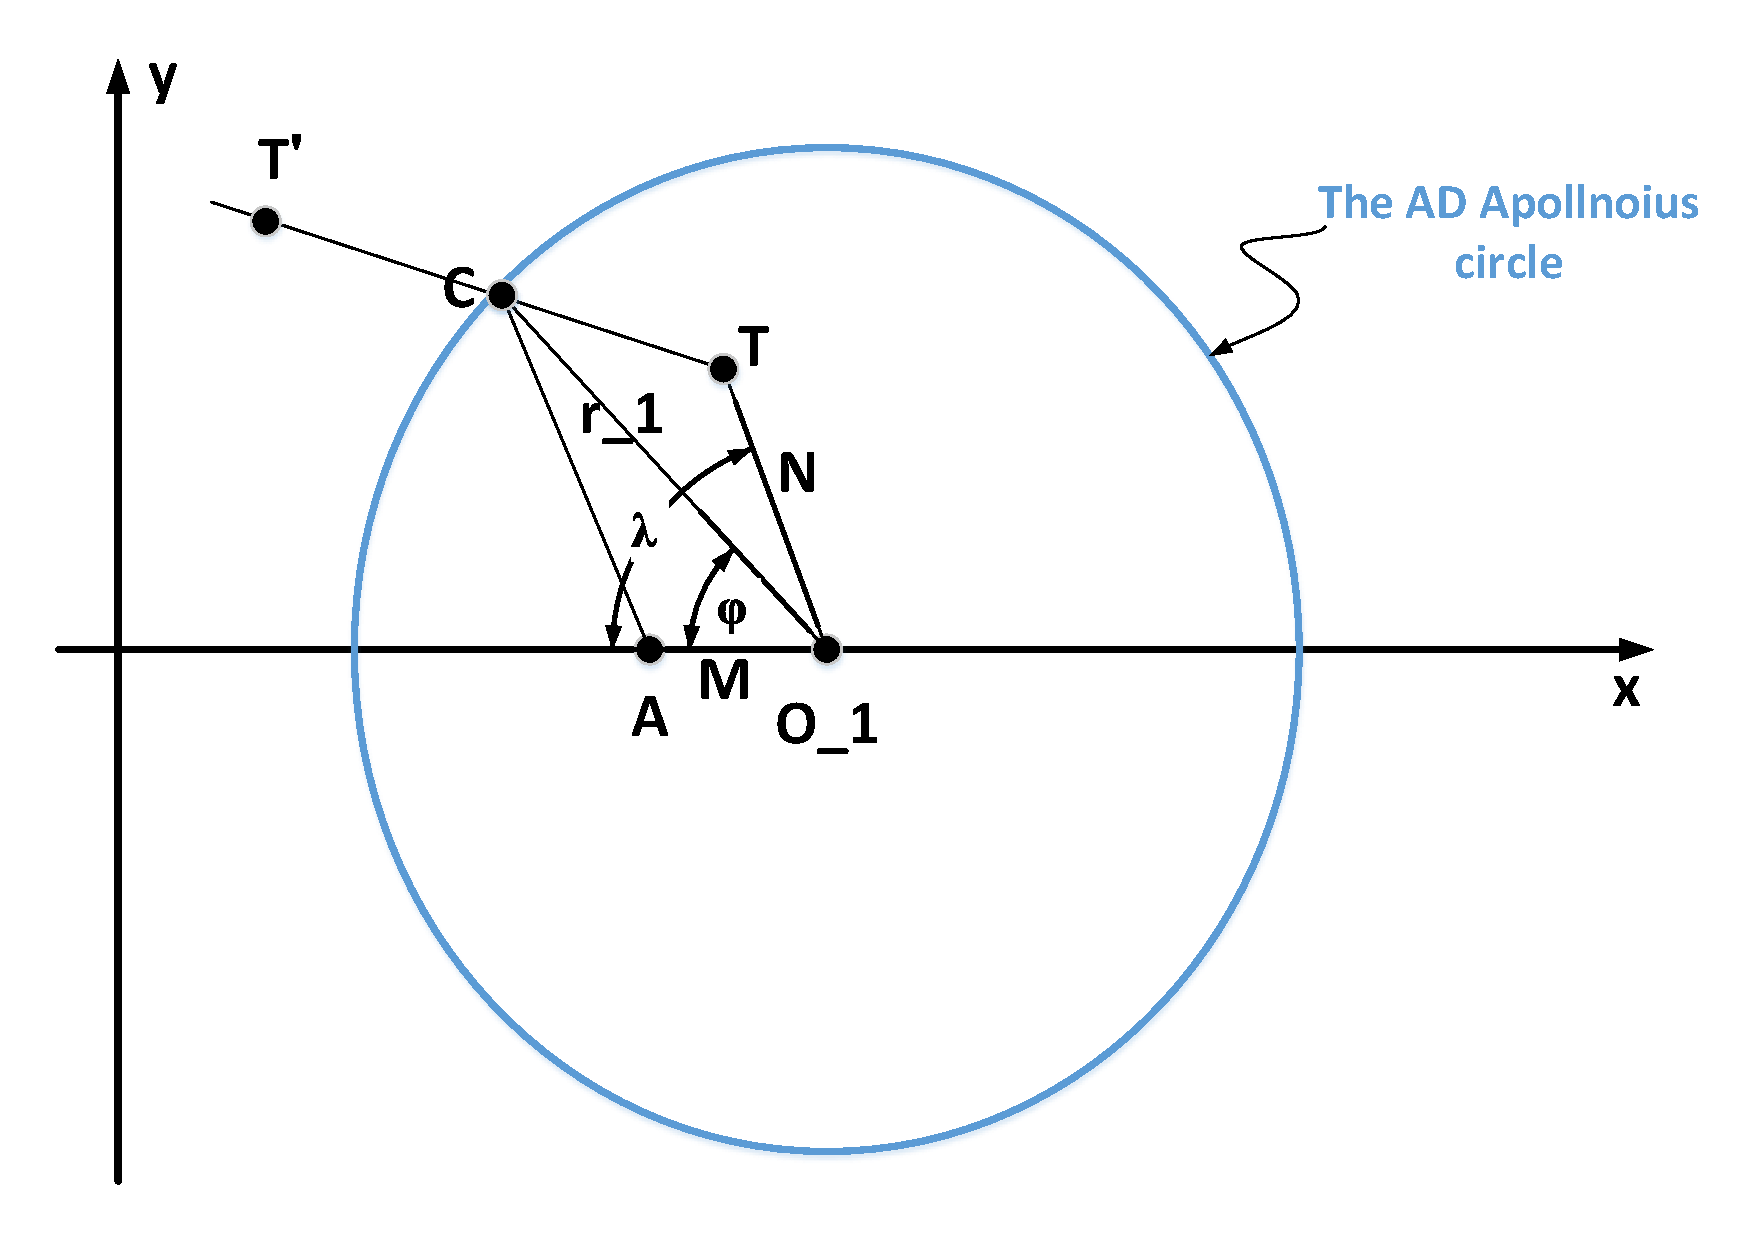
\includegraphics[width=1.0\textwidth]{fig/Drawing6_2.pdf}
\caption{Pertaining to expressing the final separation in terms of the shown distance and angles for $\gamma<1$ and $T$ inside the AD Apollonius circle, i.e., outside $R_r$.}
\label{6.2}
\end{figure}


\section{Target initial position is in the R.H.S. of the $XY$-plane, and $\gamma=1$}
This case, which appears here for the first time, resembles that of Sec. 6.1, with the exception that the condition $\gamma=1$ makes the $AD$-Apollonius circle degenerate into the perpendicular bisector or the $Y$-axis (Fig. \ref{6.3}). Now the cost/payoff function is replaced by 



\begin{equation}
\begin{split}
J(y_c) &= CT' = CT+TT' \\
&=CT+ \alpha\ AC \\
&=[x_T^2 + (y_c - y_T)^2]^{\frac{1}{2}} + \alpha [x_A^2 + y_c^2]^{\frac{1}{2}}.
\label{Jyc}
\end{split}
\end{equation} 

and one has to solve a single-variable unconstrained minimization problem.
\begin{equation}
min_{y_c}\ J(y_c)
\end{equation}

by setting $\dfrac{d J(y_c)}{d y_c}$ to zero, i.e.,

\begin{equation}
\dfrac{d J(y_c)}{d y_c} = \dfrac{(y_c - y_T)}{[x_T^2 + (y_c - y_T)^2]^{\frac{1}{2}}} + \dfrac{\alpha y_c}{[x_A^2 + y_c^2]^{\frac{1}{2}}} =0.
\label{6-24}
\end{equation}

which can be arranged as 
\begin{equation}
(y_c - y_T)(x_A^2 + y_c^2)^{\frac{1}{2}} = - \alpha y_c (x_T^2 + (y_c - y_T)^2)^{\frac{1}{2}}
\label{6-25}
\end{equation}

Equation (\ref{6-25}) can be squared to yield the following quartic (fourth-degree) real equation in $y_c$.

\begin{equation}
(y_c^2 - 2y_c y_T + y_T^2)(x_A^2 + y_c^2)
=\alpha^2 y_c^2 [x_T^2 + y_c^2 + y_T^2 - 2y_c y_T]
\label{6-26}
\end{equation}

or

\begin{equation}
(1-\alpha^2)y_c^4 - 2(1-\alpha^2) y_T y_c^3
+[(1-\alpha^2)y_T^2 + x_A^2 - \alpha^2 x_T^2]y_c^2
-2 x_A^2 y_T y_c + x_A^2 y_T^2 =0
\label{4thPoly}
\end{equation}

Equation (\ref{4thPoly}) yields four roots (expected to ba all real, or to have two real and two complex conjugate roots). Each of the real roots is substituted into $J(y_c)$ given by (\ref{Jyc}) to select the one minimizing it.

\begin{figure}[H]
\centering
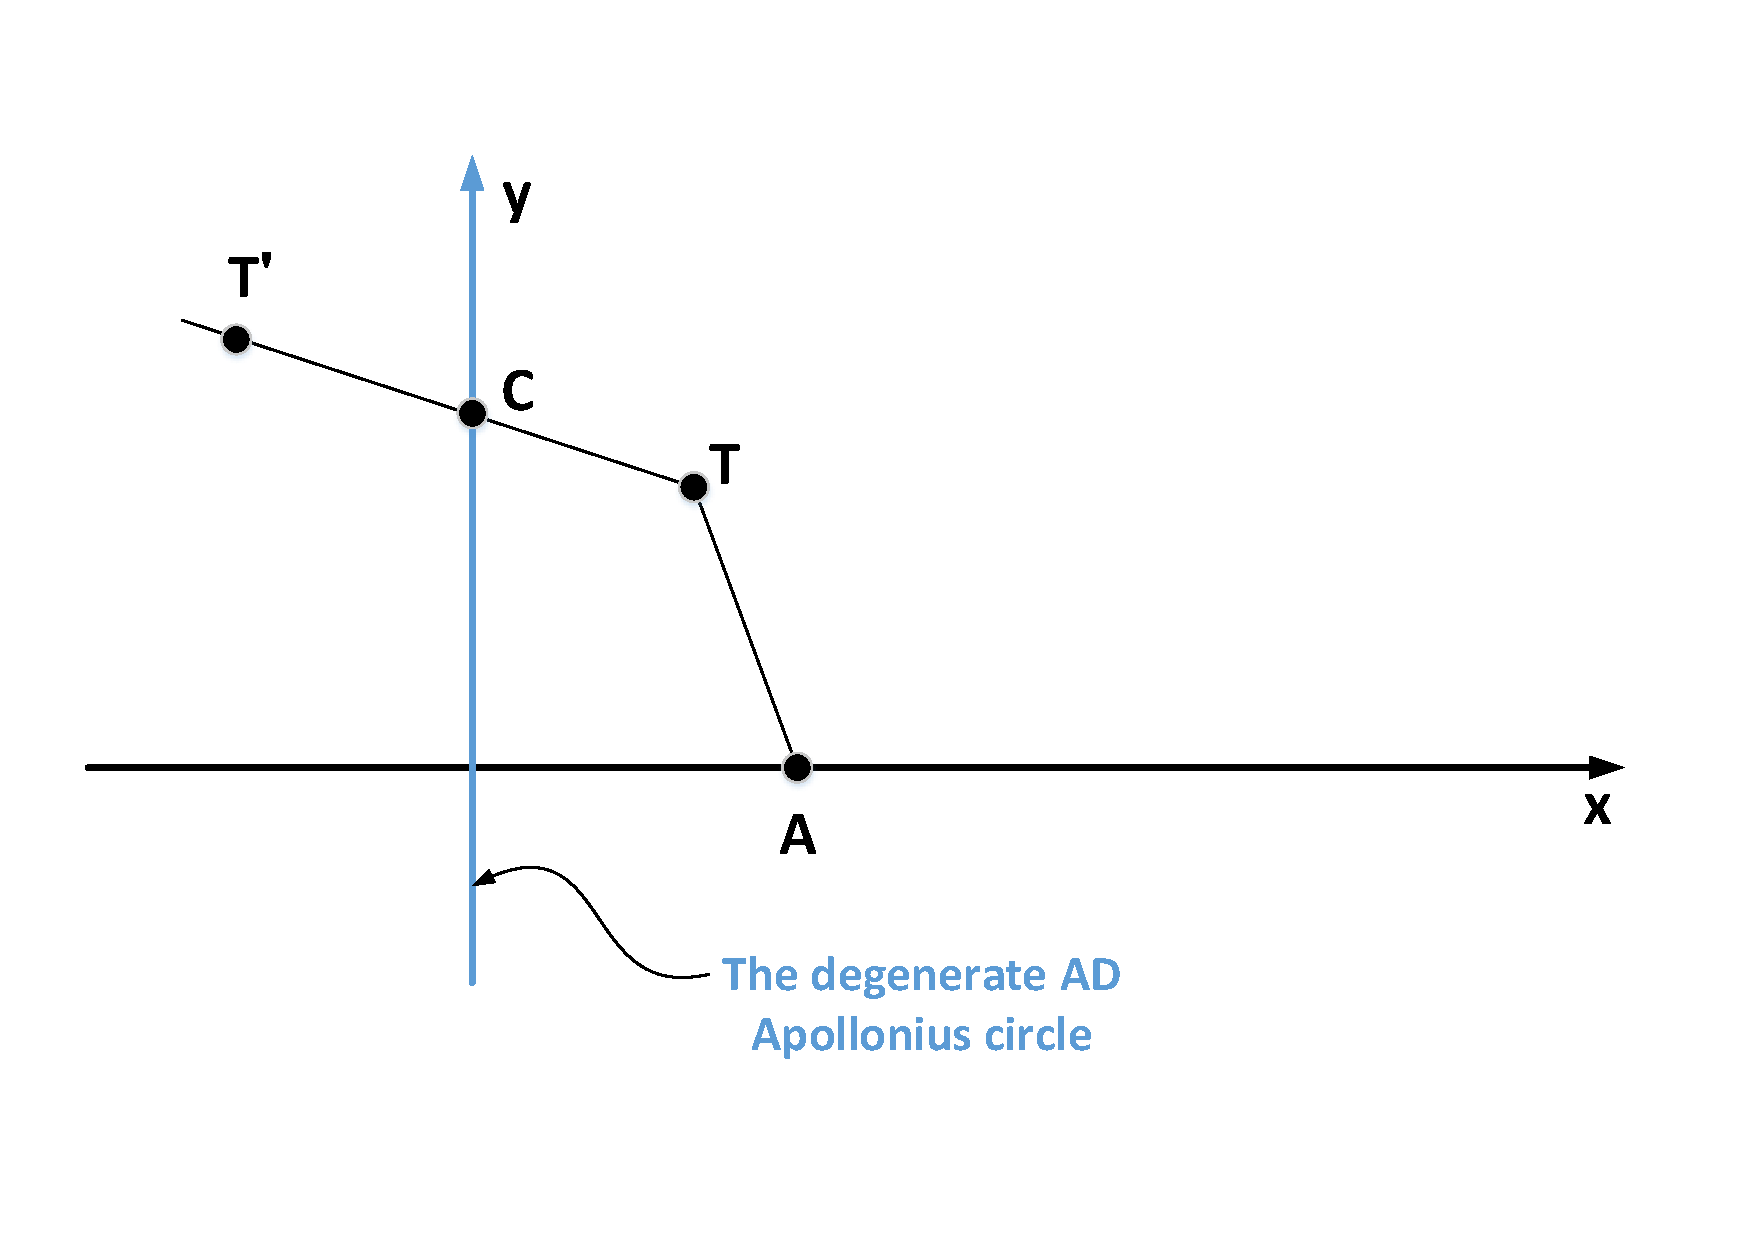
\includegraphics[width=1.0\textwidth]{fig/Drawing6_4.pdf}
\caption{Pertaining to expressing the final separation $CT'$ when $\gamma=1$ and $T$ is in the R.H.S. of the Y-plane, i.e., outside $R_r$.}
\label{6.4}
\end{figure}

\section{Target initial position is in the L.H.S. of the $XY$-plane, and $\gamma=1$}

This case was discussed previously by Garcia et al. [], and resemble that of Sec. 6.1, with the exception that the condition $\gamma=1$ makes the $AD$-Apollonius circle degenerate into the perpendicular bisector or the $Y$-axis (Fig. \ref{6.4}).
The current case is also similar to the case in Sec. 6.3, with the exception that $\boldsymbol{T}$ is in the L.H.S. rather than the R.H.S. of the $Y$-plane. Now, the cost/payoff function is replaced by 
\begin{equation}
\begin{split}
J(y_c) &= CT' = TT'-CT \\
&=\alpha\ AC -CT \\
&=\alpha [x_A^2 + y_c^2]^{\frac{1}{2}}-[x_T^2 + (y_c - y_T)^2]^{\frac{1}{2}},
\label{Jyc4}
\end{split}
\end{equation}    

and one has to solve a single-variable unconstrained maximization problem

\begin{equation}
max_{y_c}\ J(y_c)
\end{equation}
by setting $\dfrac{d J(y_c)}{d y_c}$ to zero, i.e.,
\begin{equation}
\dfrac{d J(y_c)}{d y_c} = \dfrac{\alpha y_c}{[x_A^2 + y_c^2]^{\frac{1}{2}}} - \dfrac{(y_c - y_T)}{[x_T^2 + (y_c - y_T)^2]^\frac{1}{2}}
\label{6-30}
\end{equation}
Equation (\ref{6-30}) can be rearranged and then squared to yield (\ref{6-26}) and consequently (\ref{4thPoly}). Each of the real roots or the quartic equation (\ref{4thPoly}) should be substituted into $J(y_c)$ given by (\ref{Jyc4}) to decide which of them maximize $J(y_c)$


\begin{figure}[htb]
\centering
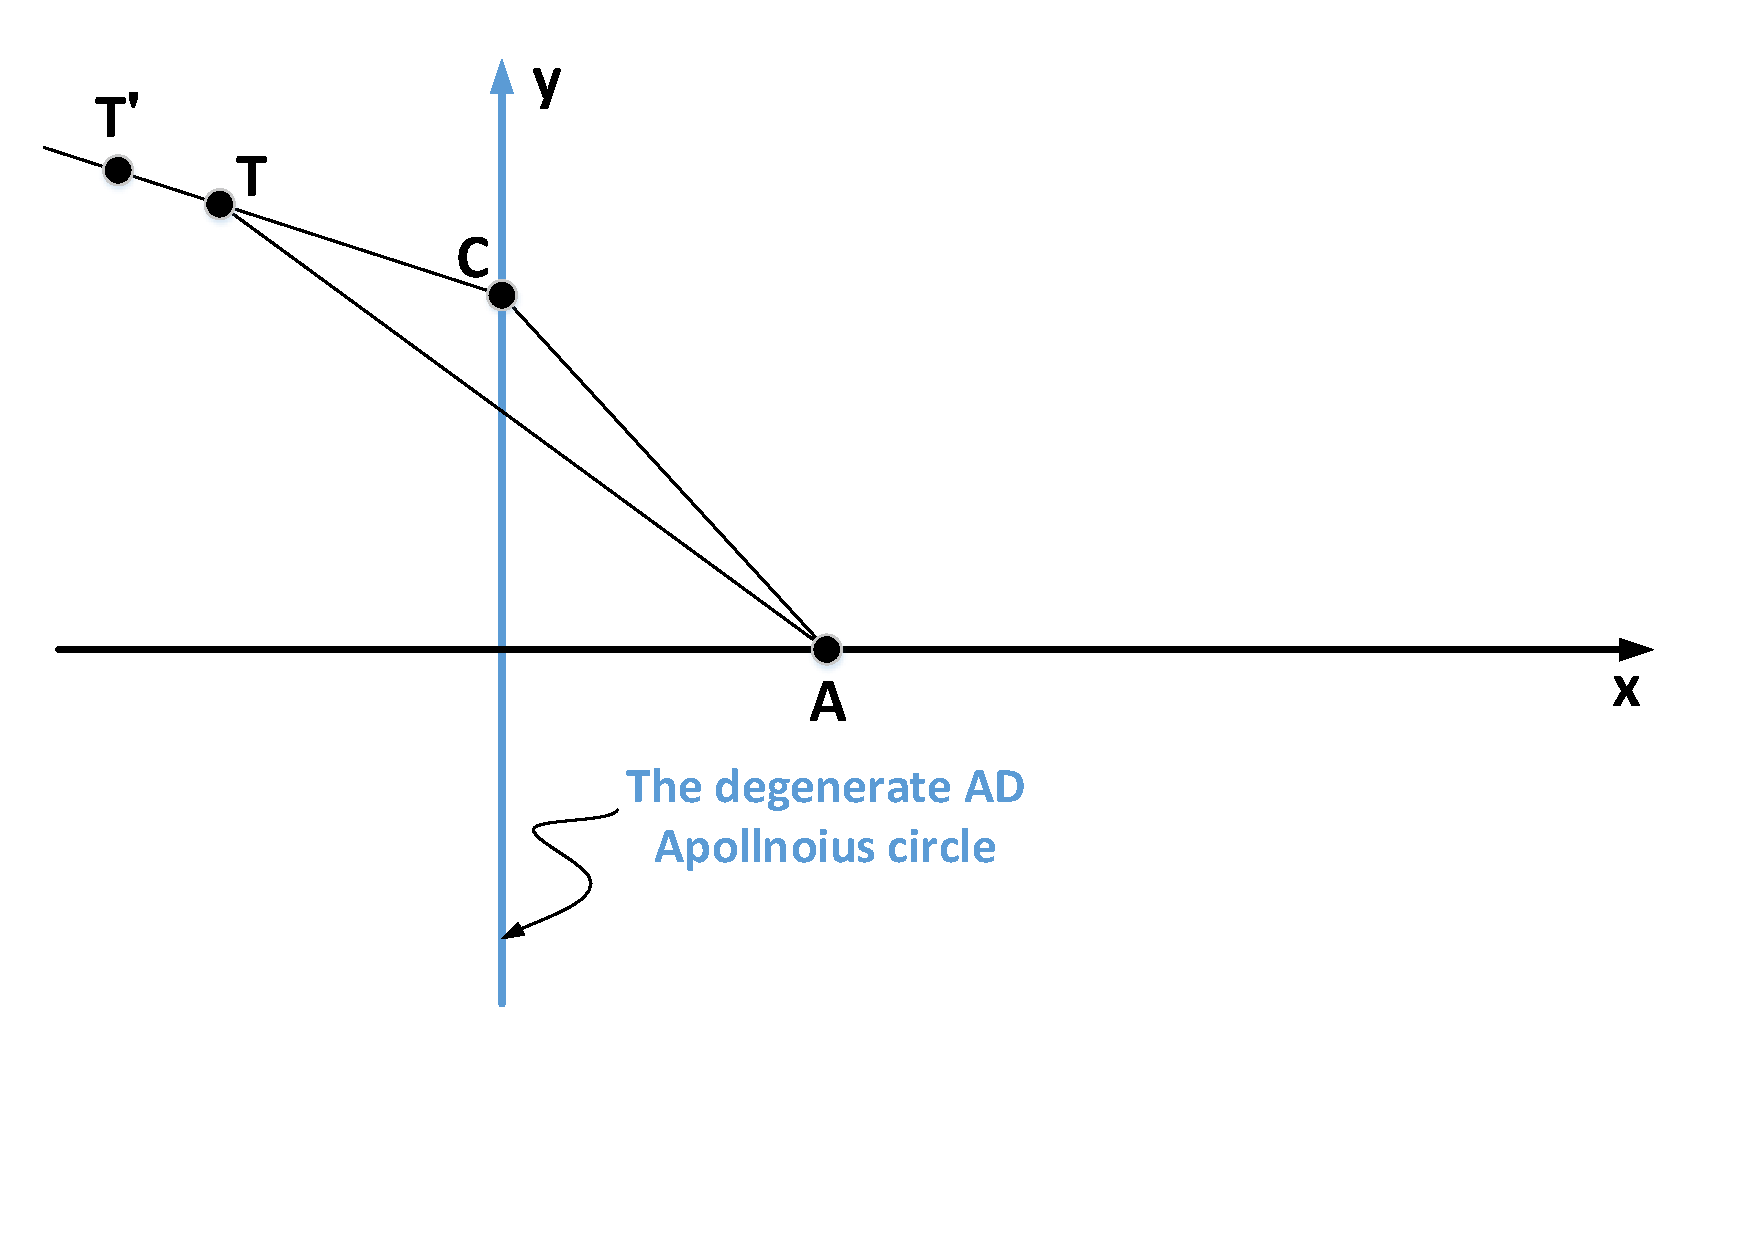
\includegraphics[width=1.0\textwidth]{fig/Drawing6_3.pdf}
\caption{Pertaining to expressing the final separation $CT'$ when $\gamma=1$ and $T$ is in the L.H.S. of the Y-plane, i.e., within $R_r$.}
\label{6.3}
\end{figure}
\section{Target initial position is inside the $AD$ Apollonius circle, and $\gamma>1$}
Again, the case discussed in this section has not appear earlier in the open literature. This case resembles the cases in sections 6.1 and 6.3 in the fact that it deals with a Target initially within $R_2$. The current situation is depicted in Fig. \ref{6.5}, in which the distances $M,\ N$ and angels $\phi$ and $\lambda$ are defined. Note that the angles $\phi$ and $\lambda$ are the polar angles (rather than complements thereof) for the position vector of $C$ and $T$ w.r.t. the center $O_1$ of the $AD$ Apollonius circle. The distance $N= O_1 T$ is still given by (\ref{N}), while $M=AO_1$ is given by 

\begin{equation}
\begin{split}
M+ AO_1 &= x_A - \dfrac{1+\gamma^2}{1-\gamma^2} x_A\\
& = \dfrac{-2 \gamma^2}{1-\gamma^2}x_A = \dfrac{2 \gamma^2}{\gamma^2 -1}x_A\\
& = \gamma r_1,
\end{split}
\end{equation}

a result that can be unified with (\ref{O11}) in the form

\begin{equation}
M= \dfrac{2 \gamma^2}{\lvert 1-\gamma^2 \rvert} x_A = \gamma r_1.
\end{equation}

with these minor observations, we can easily verify that equations (\ref{optimization prob})-(\ref{6th-poly}) are still valid in the current case.

\begin{figure}[H]
\centering
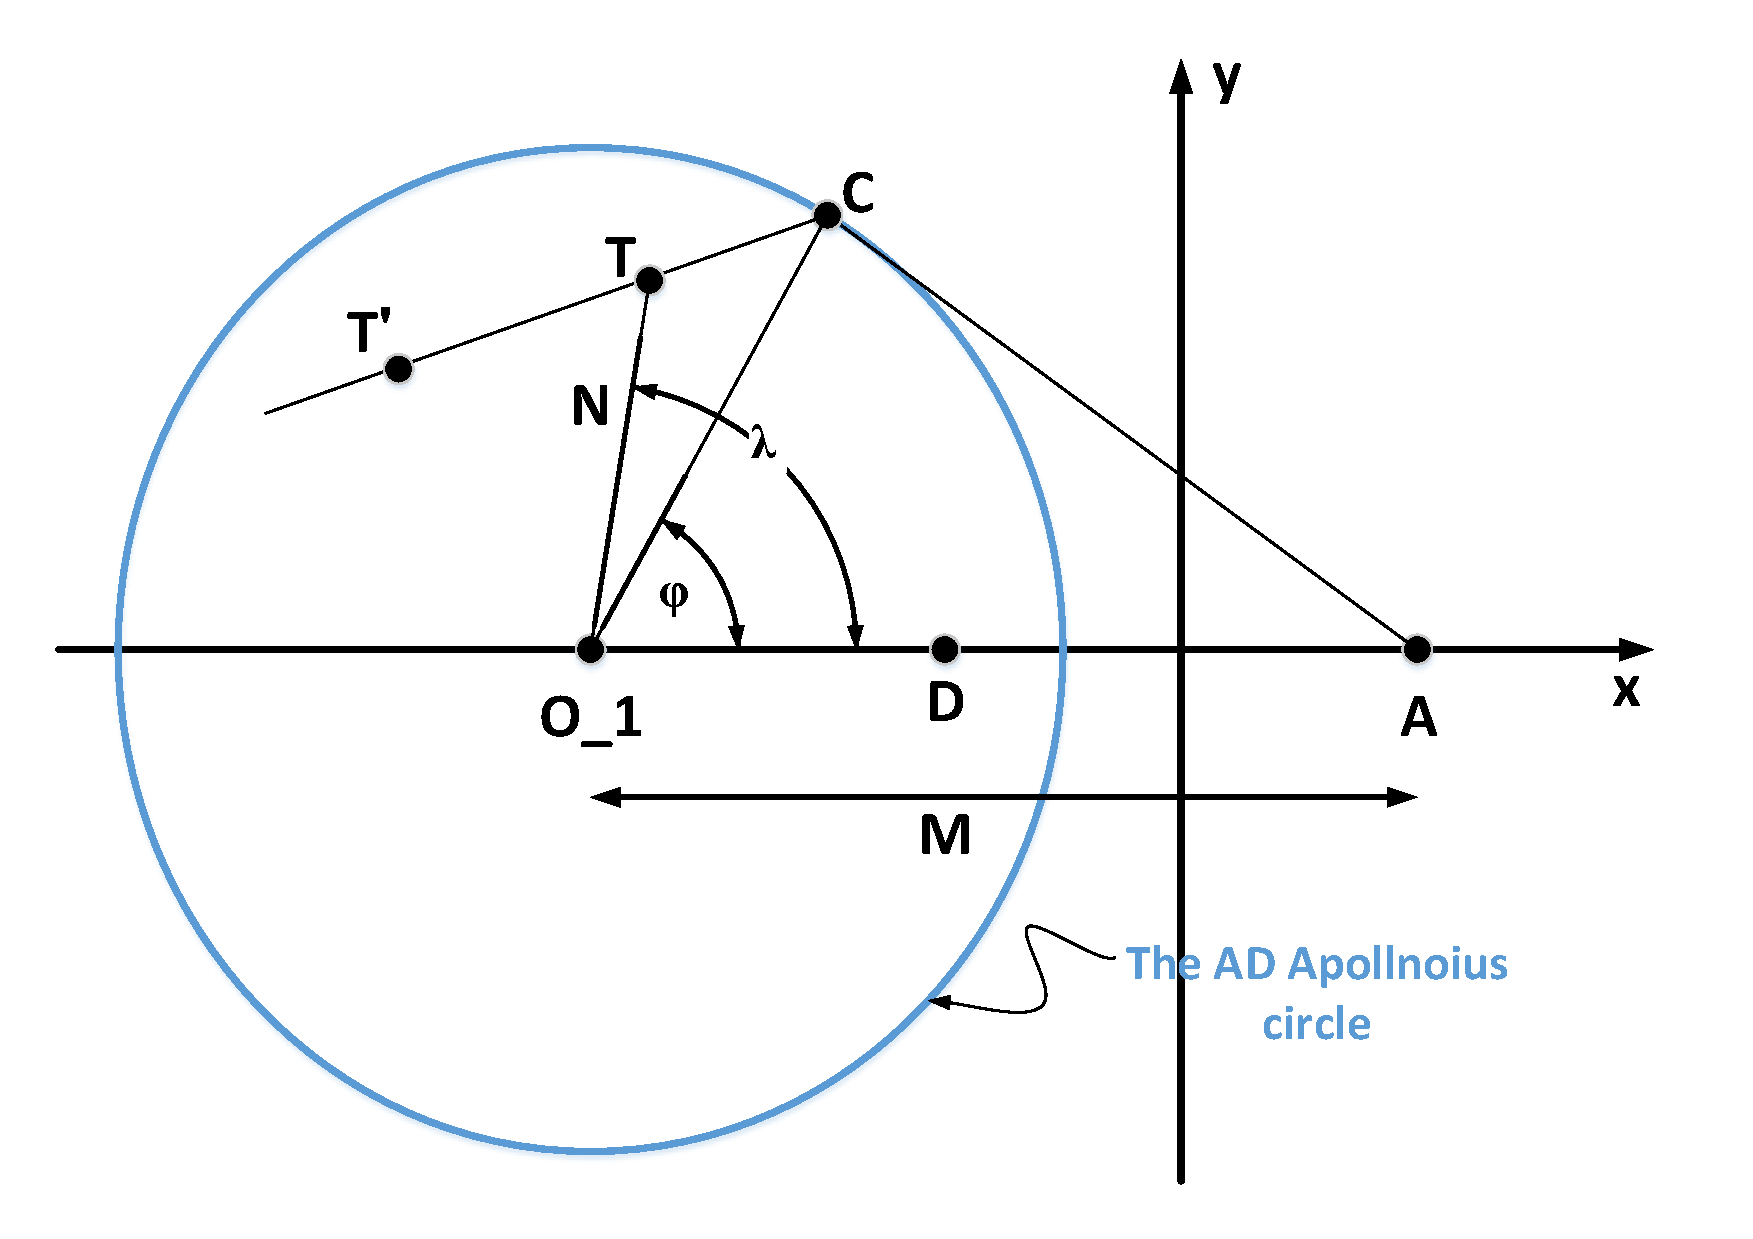
\includegraphics[width=1.0\textwidth]{fig/Drawing6_5.pdf}
\caption{Pertaining to expressing the final separation in terms of the shown distance and angles for $\gamma>1$ and $T$ inside the AD Apollonius circle, i.e., within $R_r$.}
\label{6.5}
\end{figure}

\section{Target initial position is outside the $AD$ Apollonius circle, and $\gamma>1$}
This case is again a novel case. It resembles the cases in the Sections 6.2 and 6.4 in the fact that it deals with a Target initially outside $R_r$. It is similar to the case in the previous section (Sec. 6.5) as both sections deals with a slow Defender. The situation is demonstrated by Fig. \ref{6.6}, which has similarities and differences with Fig. \ref{6.2} and Fig. \ref{6.5}. We can easily verify that equations (\ref{constrained optimization})-(\ref{cost-fun-sub2}), and consequently equations (\ref{6-14})-(\ref{6th-poly}) are still valid in the current case.

\begin{figure}[H]
\centering
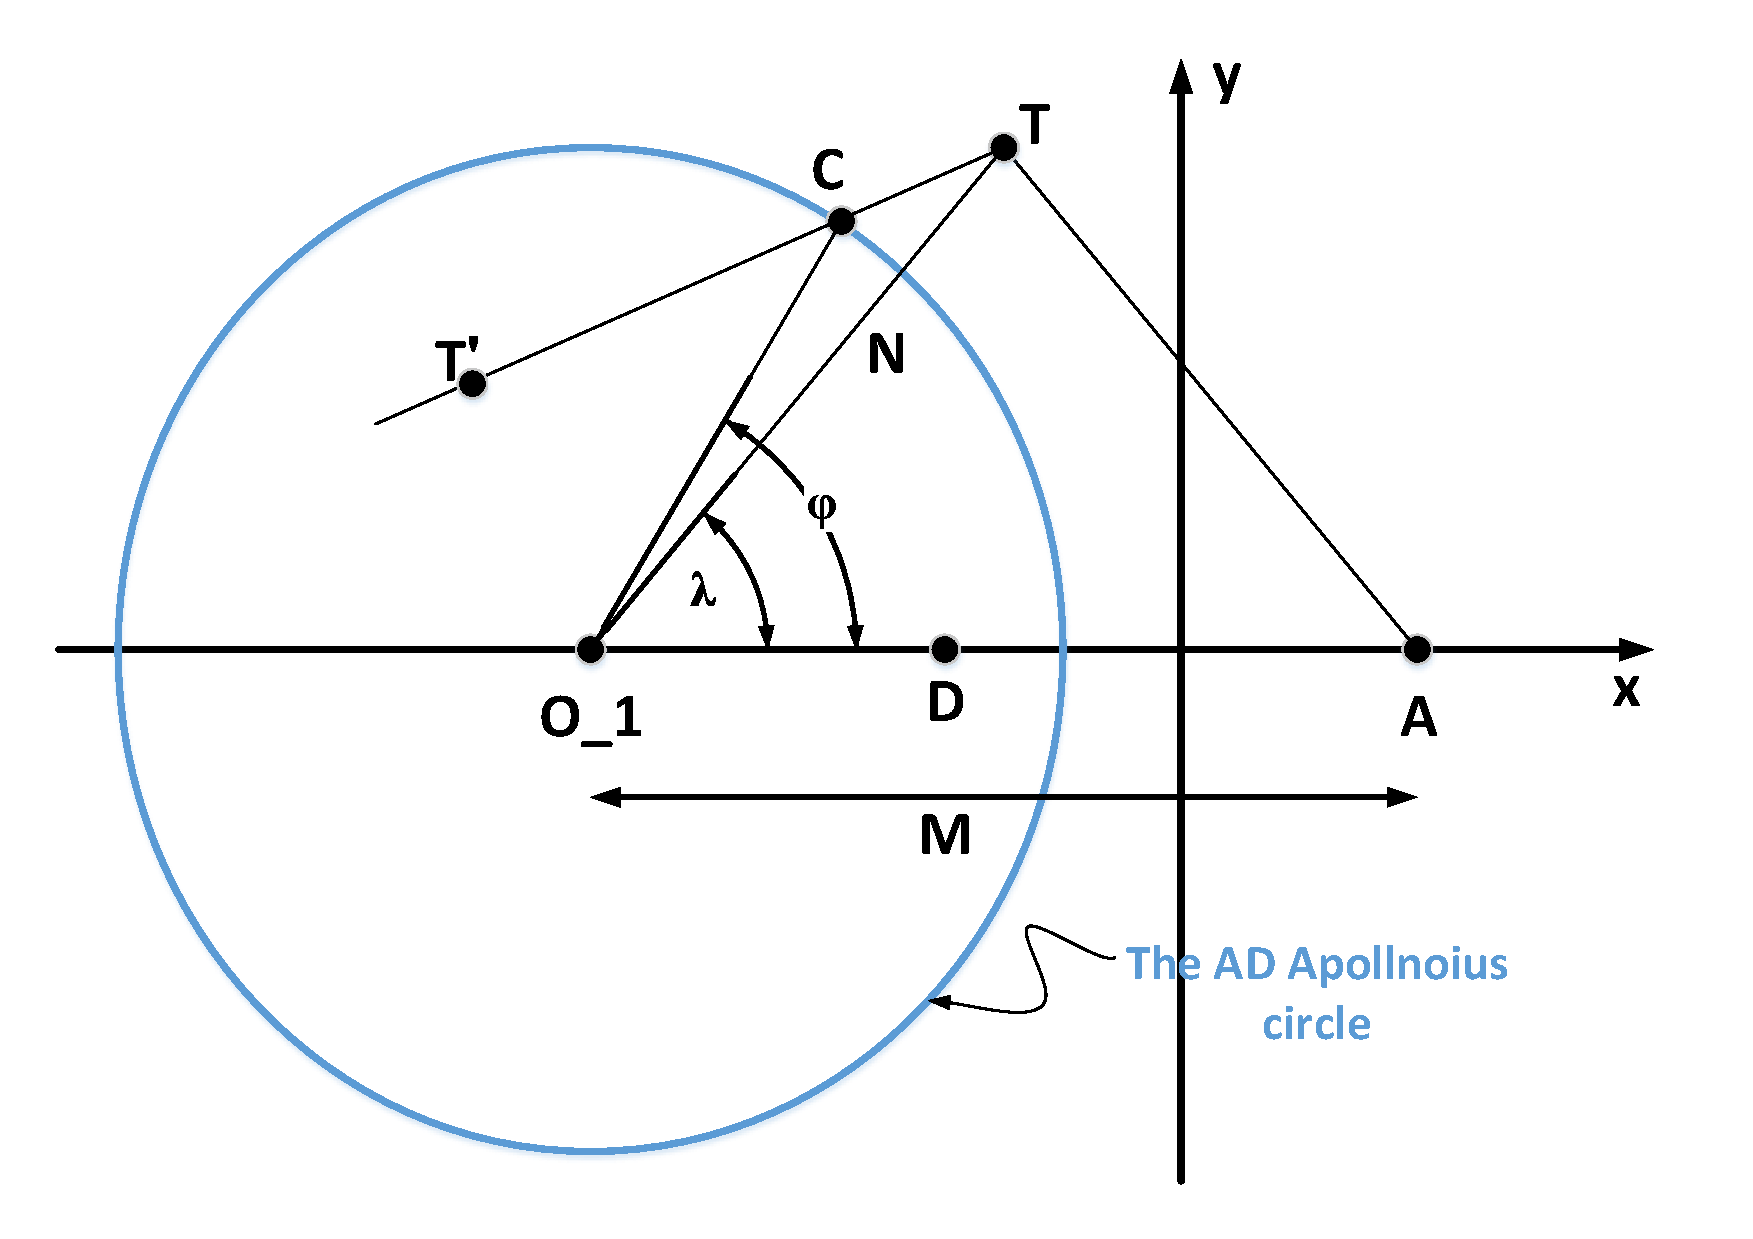
\includegraphics[width=1.0\textwidth]{fig/Drawing6_6.pdf}
\caption{Pertaining to expressing the final separation in terms of the shown distance and angles for $\gamma>1$ and $T$ outside the AD Apollonius circle, i.e., outside $R_r$.}
\label{6.6}
\end{figure}

\section{Numerical Results}
We study the optimal values of $\phi$ or $y_c$ for $x_A=4,\ \alpha=0.25$ and the following choices of $\gamma$ and $(x_T,y_T)$
\subsection{$\gamma=0.8,\ x_T=1.0,\ y_T=20.0$}
This is the case in Sec. 6.1, and is handled by obtaining six roots via (\ref{6th-poly}) and selecting the one which minimizes $J(\phi)$ in (\ref{cost-fun-sub}). Results are shown in Table 6.1 and the optimal value of $\phi$ is $\phi_{optimal}=$


\begin{center}
\begin{tabular}{ |c||c|c| } 
\hline
i & $\phi_i = Root\neq i$ of (\ref{6th-poly}) & $J(\phi_i)$ in (\ref{cost-fun-sub}) [choose minimum]  \\
 \hline
 \hline
 1 &  &  \\
 \hline 
 2 &  &  \\
 \hline 
 3 &  &  \\ 
 \hline
 4 &  &  \\
  \hline
  5&  &  \\ 
   \hline
   6 &  &  \\  
  \hline
\end{tabular}
%\caption{Optimal strategy for a case of Section 6.1 $(\gamma=0.8,\ x_T=1,\ y_T=20)$}
%\label{table6.1}
\end{center}


\subsection{$\gamma=0.8,\ x_T=20.0,\ y_T=1.0$}
This is the case in Sec. 6.2, and is handled by obtaining six roots via (\ref{6th-poly}) and selects the one that maximizes $J(\phi)$ in (\ref{cost-fun-sub2}). Results are shown in Table 6.2, and the optimal value of $\phi$ is $\phi_{optimal}=$


\begin{center}
\begin{tabular}{ |c||c|c| } 
\hline
i & $\phi_i = Root\neq i$ of (\ref{6th-poly}) & $J(\phi_i)$ in (\ref{cost-fun-sub2}) [choose minimum]  \\
 \hline
 \hline
 1 &  &  \\
 \hline 
 2 &  &  \\
 \hline 
 3 &  &  \\ 
 \hline
 4 &  &  \\ 
  \hline
 5 &  &  \\
  \hline
 6 &  &  \\
  \hline
\end{tabular}
%\caption{Optimal strategy for a case of Section 6.2 $(\gamma=0.8,\ x_T=20,\ y_T=1)$}
%\label{table6.1}
\end{center}


\subsection{$\gamma=1.0,\ x_T=-1.0,\ y_T=1.0$}
This is the case in Sec. 6.3, and is handled by obtaining four roots via (\ref{4thPoly}) and selecting the one that \textit{minimizes} $J(\phi)$ in (\ref{6-24}). Results are shown in Table 6.3, and the optimal value of $y_c=$

\begin{center}
\begin{tabular}{ |c||c|c| } 
\hline
i & $\phi_i = Root\neq i$ of (\ref{cost-fun-sub2}) & $J(\phi_i)$ in (\ref{6-24}) [choose minimum]  \\
 \hline
 \hline
 1 &  &  \\
 \hline 
 2 &  &  \\
 \hline 
 3 &  &  \\ 
 \hline
 4 &  &  \\ 
  \hline
\end{tabular}
%\caption{Optimal strategy for a case of Section 6.3 $(\gamma=1,\ x_T=-1,\ y_T=1)$}
%\label{table6.3}
\end{center}

\subsection{$\gamma=1.0,\ x_T=1.0,\ y_T=1.0$}
This is the case in Sec. 6.4, and is handled by obtaining four roots via (\ref{4thPoly}) and selecting the one that maximizes $J(y_c)$ in (\ref{Jyc4}). Results are shown in Table 6.4, and the optimal value of $y_c=$

\begin{center}
\begin{tabular}{ |c||c|c| } 
\hline
i & $y_i = Root\neq i$ of (\ref{4thPoly}) & $J(\phi_i)$ in (\ref{Jyc4}) [choose minimum]  \\
 \hline
 \hline
 1 &  &  \\
 \hline 
 2 &  &  \\
 \hline 
 3 &  &  \\ 
 \hline
 4 &  &  \\ 
  \hline
\end{tabular}
%\caption{Optimal strategy for a case of Section 6.3 $(\gamma=1,\ x_T=1,\ y_T=1)$}
%\label{table6.4}
\end{center}



\subsection{$\gamma=1.25,\ x_T=-20.0,\ y_T=1.0$}
This is the case in Sec. 6.5, and is handled by obtaining six roots via (\ref{6th-poly}) and selecting the one that \textit{minimizes} $J(\phi)$ in (\ref{cost-fun-sub}). Results are shown in Table 6.5 and the optimal value of $\phi$ is $\phi_{optimal}=$


\begin{center}
\begin{tabular}{ |c||c|c| } 
\hline
i & $\phi_i = Root\neq i$ of (\ref{6th-poly}) & $J(\phi_i)$ in (\ref{cost-fun-sub}) [choose minimum]  \\
 \hline
 \hline
 1 &  &  \\
 \hline 
 2 &  &  \\
 \hline 
 3 &  &  \\ 
 \hline
 4 &  &  \\
  \hline
  5&  &  \\ 
   \hline
   6 &  &  \\  
  \hline
\end{tabular}
%\caption{Optimal strategy for a case of Section 6.5 $(\gamma=1.25,\ x_T=-20,\ y_T=1)$}
%\label{table6.5}
\end{center}




\subsection{$\gamma=1.25,\ x_T=-1.0,\ y_T=20.0$}
This is the case in Sec. 6.6, and is handled by obtaining six roots via (\ref{6th-poly}) and selecting the one that maximizes $J(\phi)$ in (\ref{cost-fun-sub2}). Results are shown in Table 6.6, and the optimal value of $\phi$ is $\phi_{optimal}=$

\begin{center}
\begin{tabular}{ |c||c|c| } 
\hline
i & $\phi_i = Root\neq i$ of (\ref{6th-poly}) & $J(\phi_i)$ in (\ref{cost-fun-sub2}) [choose minimum]  \\
 \hline
 \hline
 1 &  &  \\
 \hline 
 2 &  &  \\
 \hline 
 3 &  &  \\ 
 \hline
 4 &  &  \\
  \hline
  5&  &  \\ 
   \hline
   6 &  &  \\  
  \hline
\end{tabular}
%\caption{Optimal strategy for a case of Section 6.6 $(\gamma=1.25,\ x_T=-1,\ y_T=20)$}
%\label{table6.6}
\end{center}
